\documentclass[slug=CS, room=Andreas-Schubert-Bau\,\ Labor\ 406,
supervisor=Juliane\ Volkmer, coursedate=29.\ 11.\ 2019]{../../Lab_Report_LaTeX/lab_report}

\title{Comptonstreuung}
\author{Oliver Matthes, Valentin Boettcher}
\usepackage[version=4]{mhchem}
\usepackage{todonotes}
\graphicspath{ {figs/} }
\newcommand{\cs}{\emph{Comptonstreuung }}
\usepackage{circuitikz}
\usepackage{subcaption}
\usepackage{ amssymb }
\usepackage{tabularx}
\usepackage{pgf}
\sisetup{math-celsius = {}^{\circ}\kern-\scriptspace C}
\usepackage[ngerman]{babel}

% bib
\addbibresource{protokoll.bib}

\begin{document}
\maketitle

\section{Einleitung}
\label{sec:einl}

\cs ist in einem Energiebereich von hundert Kiloelektronenvolt bis hin zu wenigen
Megaelektronenvolt der Wechselwirkungsprozess zwischen Photonen und Materie, der am
 wahrscheinlichsten auftritt und deswegen in vielen physikalischen Bereichen beachtet werden muss.
Neben \cs gibt es natürlich auch noch andere Wechselwirkungsprozesse wie der
Photoeffekt, der vor allem bei geringen Photonenenergien auftritt oder die Paarbildung bei
der man Energien von mindestens zwei Elektronenmassen braucht, um ein Elektron-Positron-Paar
zu erzeugen. Diese Prozesse werden in diesem Versuch allerdings nicht betrachtet.\\

Um Aussagen über die Wahrscheinlichkeit, dass ein Photon mit einem Elektron wechselwirkt,
treffen zu können, definiert man den Wirkungsquerschnitt:

\begin{equation}\label{eq:wirkquer}
	\sigma = \frac{N}{\Phi}
\end{equation}

\begin{tabular}{llll}
	 & \(N\)    & ... & mittlere Wechselwirkungsanzahl eines Teilchens mit einem atomaren Target \\
	 & \(\Phi\) & ... & Teilchenfluenz, dem das Target ausgesetzt ist
\end{tabular}\\

Der Wechselwirkungsquerschnitt der inkohärenten Streuung und damit des Comptoneffekts ist
proportional zur Ordnungszahl des Atoms (\(\sigma_i \propto\) Z).\\

\subsection{Inkohärente Streuung}
\label{sec:inkostreu}

Wichtig, um \cs beschreiben zu können, ist der Prozess der \emph{inkohärenten Streuung}.
Dabei überträgt das Photon bei der Wechselwirkung mit einem an einem Atomkern gebundenen
Elektron einen Teil seiner Energie auf dieses, so dass es den gebundenen Zustand verlassen kann.
Vernachlässigt man bei diesem Prozess die Bindungsenergie des Elektrons, nennt man diesen \cs,
da Arthur Holly Compton 1922 diese Annahme traf, um diesen Effekt zu beschreiben.\\

\subsubsection{Comptonstreuung}
\label{sec:cs}

Um \cs zu beschreiben, geht man, wie oben schon erwähnt, von quasi freien Elektronen aus.
Diese Annahme trifft besonders gut auf Metalle zu (im Experiment werden wir mit einem Aluminiumtarget arbeiten).
Wird ein Photon an einem Elektron gestreut, ändert sich seine Energie sowie seine 
Bewegungsrichtung um einen polaren Streuwinkel \(\vartheta\). Nutzt man den Energie-
und den Impulserhaltungssatz aus und setzt den Photonenimpuls \(p = E/c\) ein, so erhält man
einen Ausdruck für die Energie des Wechselwirkungsphotons nach der Interaktion:

\begin{gather}
	E(\mu) = \frac{E'}{1 + \kappa(1 - \mu)} \label{eq:photoenergie}\\
	\kappa = \frac{E'}{m_0c^2}\\
	\mu = \cos\vartheta
\end{gather}

\begin{tabular}{llll}
	& \(E'\)    & ... & Photonenenergie vor dem Stoß
\end{tabular}\\

Die Ruheenergie des Elektrons beträgt:

\begin{equation}\label{key}
	E_{e^-} = m_0c^2 = \SI{511}{\kilo\electronvolt}
\end{equation}\\

Die maximal mögliche Energie, die ein Photon nach der Streuung haben kann, ist also dessen
Ausgangsenergie. Bei einem Streuwinkel von \(\vartheta = 0^\circ\) (Vorwärtsstreuung) folgt
\(\mu \rightarrow 1 \implies E(\mu) \rightarrow E'\).
Die Minimalenergie wird bei \(\mu = -1\), also bei \(\vartheta = 180^\circ\), erreicht, da
hier gilt:

\begin{equation}\label{eq:emax}
	E(\mu) = \frac{E'}{1 + 2\kappa}
\end{equation}

Je größer der polare Streuwinkel \(\vartheta\) des Photons ist, desto mehr Energie wird beim Stoß
an das Elektron übertragen. Je größer außerdem die Ausgangsenergie des Photons, desto größer ist
der Energieverlust bei der Streuung und desto höher ist zudem die Winkelabhängigkeit des
Energieverlustes (vgl.~\ref{fig:evontheta}).\\

\begin{figure}[H]\centering
	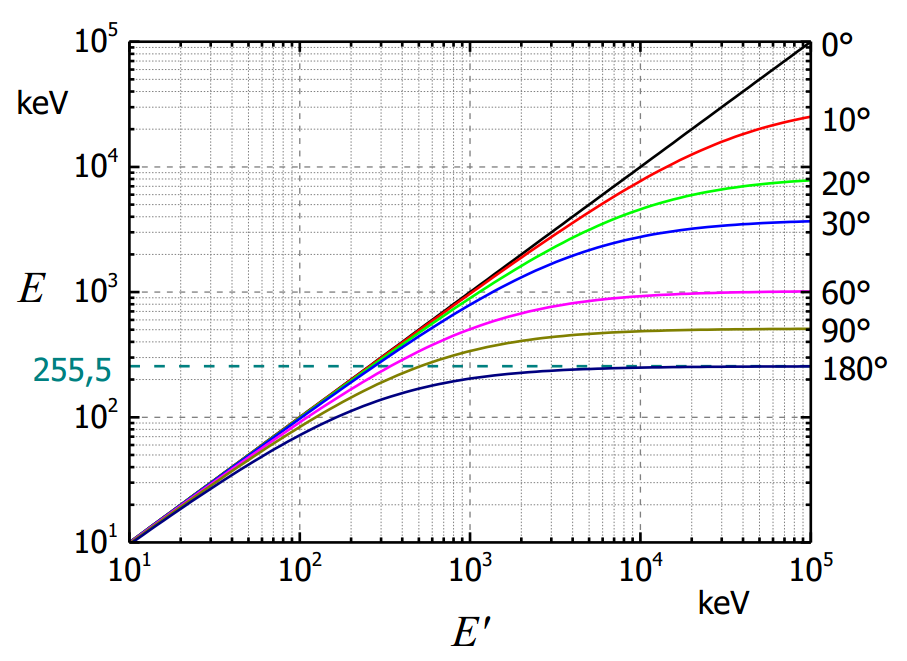
\includegraphics[width=.5\columnwidth]{./pictures/evontheta.png}
	\caption{Abhängigkeit der Energien vor und nach dem Stoß \(E'\) und \(E\) vom Streuwinkel
	\(\vartheta\).}
	\label{fig:evontheta}
\end{figure}

Um eine Aussage zur Wahrscheinlichkeit zu treffen, mit der ein Photon in einem Raumwinkelelement
\(d\Omega = \sin\vartheta d\vartheta d\phi\) gestreut wird, haben \textsc{O. Klein} und
\textsc{Y. Nishina} 1929 einen analytischen Ausdruck für den differentiellen Wirkungsquerschnitt
hergeleitet:

\begin{equation}\label{eq:kn}
	\sigma^{\text{KN}}_\Omega(\mu) = \frac{d\sigma}{d\Omega} = \frac{r_e^2}{2} \cdot \qty(\frac{1}{1 + \kappa(1 - \mu)})^2 \cdot \qty(\kappa(1 - \mu) + \frac{1}{1 + \kappa(1 - \mu)} + \mu^2)
\end{equation}

Mit \(r_e = \SI{2,818e-15}{\metre}\) als klassischen Elektronenradius.\\

Für \(\mu = 1\), also Vorwärtsstreuung folgt:
\begin{equation}\label{key}
	\sigma^{\text{KN}}_\Omega(\mu = 1) = r_e^2 = \SI{79,4}{\milli\barn}
\end{equation}

\begin{figure}[H]\centering
	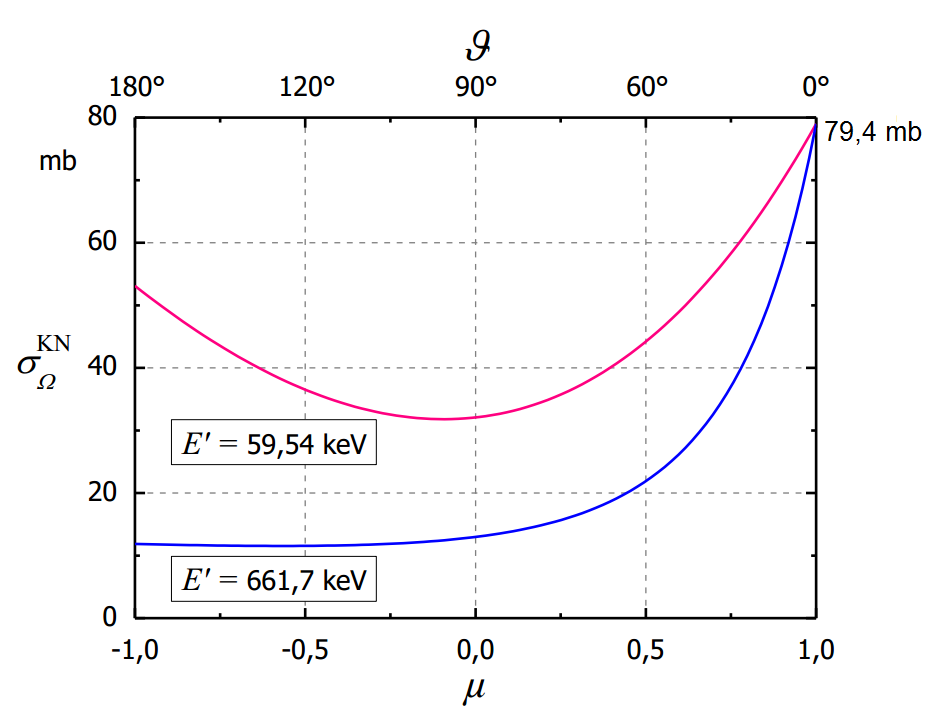
\includegraphics[width=.5\columnwidth]{./pictures/sigma_kn.png}
	\caption{\(\sigma^{\text{KN}}_\Omega(\mu)\) für verschiedene \(E'\).}
	\label{fig:sigmakn}
\end{figure}

\subsubsection{Korrektur für inkohärente Streuung}
\label{sec:cskorrektur}

Wenn man die Bindungsenergie der Elektronen nicht vernachlässigt, multipliziert man zur
Korrektur des differentiellen Wirkungsquerschnitts an die \textsc{Klein}-\textsc{Nishina}-Formel
eine inkohärente Streufunktion \(S(E', \mu, Z)\) dran:

\begin{equation}\label{eq:knkorrektur}
	\sigma^{i}_\Omega(E', \mu, Z) = \sigma^{\text{KN}}_\Omega(E', Z) \cdot S(E', \mu, Z)
\end{equation}

Es gilt, dass \(\sigma^{i}_\Omega < \sigma^{\text{KN}}_\Omega\). Insbesondere geht 
\(\sigma^{i}_\Omega\) bei \(\vartheta \rightarrow 0\) ebenfalls gegen Null, was man damit erklären
kann, dass bei \(\vartheta \rightarrow 0\) die vom Photon auf das Elektron übertragene Energie
gegen Null konvergiert, sodass diese irgendwann die Elektronenbindungsenergie unterschreitet,
das Elektron also auch nach der Interaktion mit dem Photon gebunden bleibt und somit keine
inkohärente Streuung mehr vorliegt (vgl.~\ref{fig:sigmaknkorrigiert}).

\begin{figure}[H]\centering
	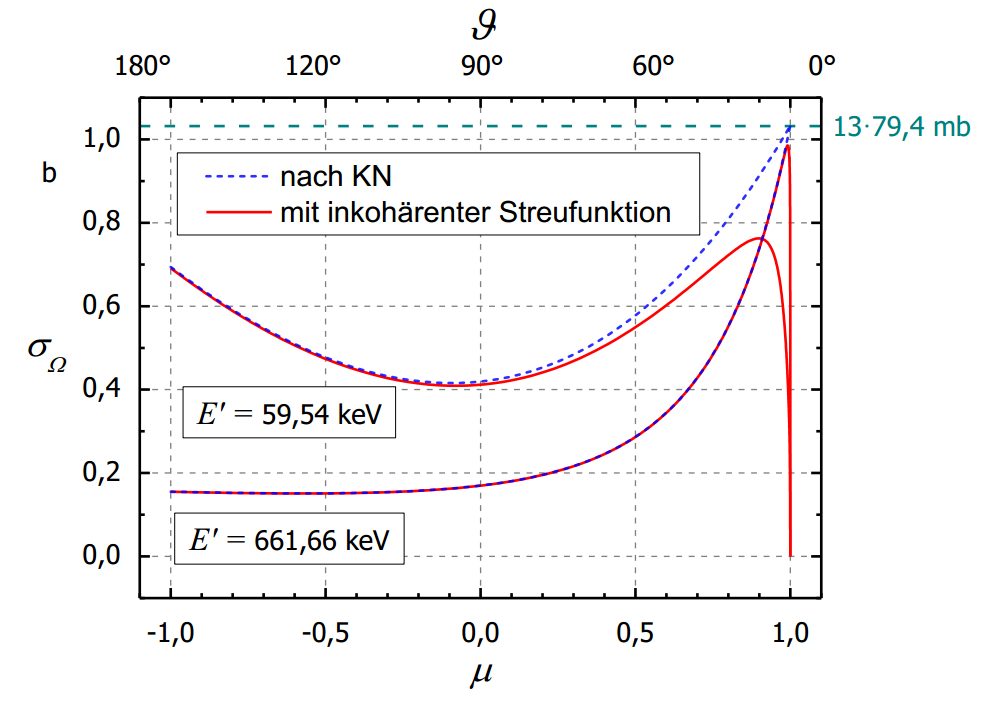
\includegraphics[width=.5\columnwidth]{./pictures/sigma_kn_korrigiert.png}
	\caption{Gegenüberstellung von \(\sigma^{i}_\Omega\) und \(\sigma^{\text{KN}}_\Omega\) für
	Aluminium und verschiedene \(E'\).}
	\label{fig:sigmaknkorrigiert}
\end{figure}

\section{Durchführung und Auswertung}
\label{sec:experiment}

Der Versuchsaufbau war wie in der Versuchsanleitung beschrieben, nur zeigte die Strahlrichtung
stets gen Wand. Außerdem wurde ein Szintillationsdetektor statt, wie in~\ref{fig:versuchsaufbau}
zu sehen, eines Halbleiterdetektors verwendet.

\begin{figure}[H]\centering
	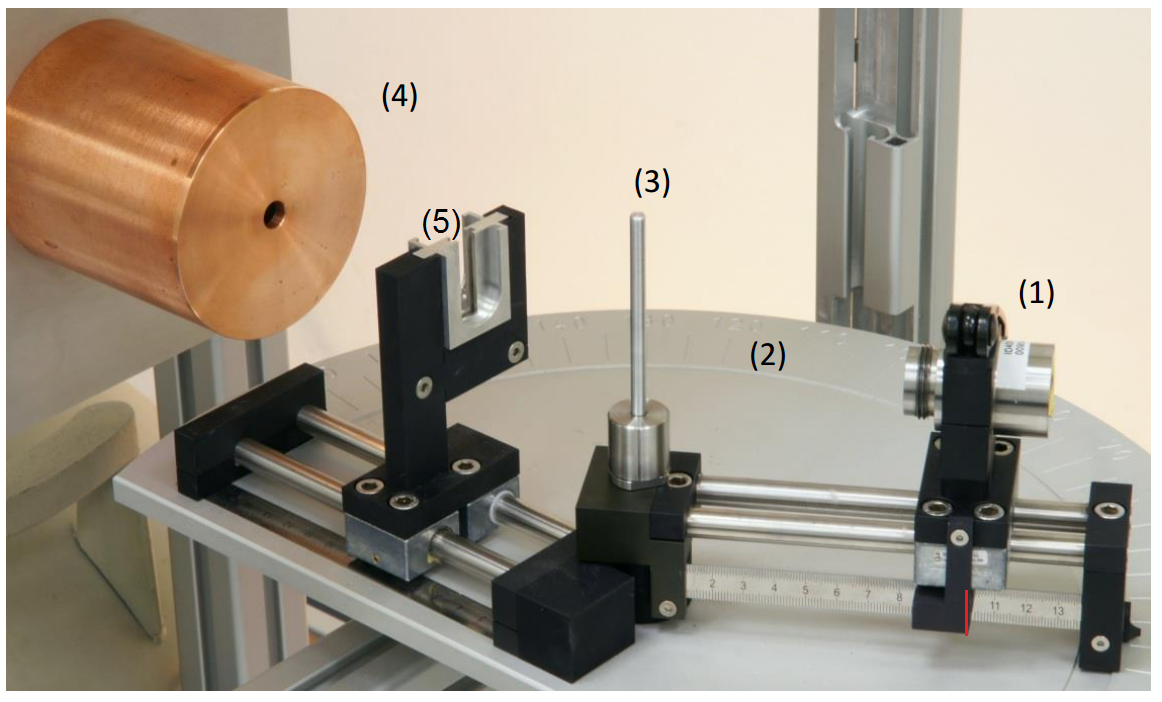
\includegraphics[width=.7\columnwidth]{./pictures/versuchsaufbau.png}
	\caption{Ähnlicher Versuchsaufbau, da ein ähnlich aussehender Szintillationsdetektor anstelle 
		des hier abgebildeten Halbleiterdetektors (4) verwendet wurde.}
	\label{fig:versuchsaufbau}
\end{figure}

Der in~\ref{fig:versuchsaufbau} dargestellte Versuchsaufbau bestand aus folgenden Komponenten:
(1) Halterung für die kollimierte \(^{241}\)Am-Probe, dessen Abstand zum Aluminiumprobenstab (3)
variiert und mit Hilfe eines angebrachten Maßstabes zu \(\approx \SI{2}{\milli\metre}\)
Genauigkeit abgelesen werden konnte. Der Abstand wurde an der unteren rechten Seite (roter Strich
in~\ref{fig:versuchsaufbau}) abgelesen. Der Streuwinkel konnte variiert und mittels eines
Goniometers (2), das aller \(5^\circ\) einen Strich hatte, auf \(\approx 2^\circ\) genau
eingestellt werden. In den Probenhalter (5) wurden für die Kalibrierung des Detektors drei
verschiedene Probenscheiben in die zum Detektor zeigende Seite eingesetzt und dieser so nah wie
möglich an den Detektor herangeschoben, um für eine, am Anfang auf \(\SI{20}{\min}\) festgesetzte,
Messzeit, möglichst viele Ereignisse zu zählen.

\subsection{Kalibrierung des Detektors}
\label{sec:kalib}

Für die Detektorkalibrierung wurden drei verschiedene Probenscheiben aus \(^{137}\)Cs, 
\(^{133}\)Ba und \(^{152}\)Eu sowie die eigentliche \(^{241}\)Am-Probe verwendet.

\section{Verzeichnisse}

\label{sec:literatur}

\listoffigures

\listoftables

\printbibliography
\end{document}